%definira klasu dokumenta 
\documentclass[12pt]{report} 

%prostor izmedu naredbi \documentclass i \begin{document} se zove uvod. U njemu se nalaze naredbe koje se odnose na cijeli dokument

%osnovni LaTex ne može riješiti sve probleme, pa se koriste različiti paketi koji olakšavaju izradu željenog dokumenta
\usepackage[croatian]{babel} 
\usepackage{amssymb}
\usepackage{amsmath}
\usepackage{txfonts}
\usepackage{mathdots}
\usepackage{titlesec}
\usepackage{array}
\usepackage{lastpage}
\usepackage{etoolbox}
\usepackage{tabularray}
\usepackage{color, colortbl}
\usepackage{adjustbox}
\usepackage{geometry}
\usepackage[classicReIm]{kpfonts}
\usepackage{hyperref}
\usepackage{fancyhdr}

\usepackage{float}
\usepackage{setspace}
\restylefloat{table}


\patchcmd{\chapter}{\thispagestyle{plain}}{\thispagestyle{fancy}}{}{} %redefiniranje stila stranice u paketu fancyhdr

%oblik naslova poglavlja
\titleformat{\chapter}{\normalfont\huge\bfseries}{\thechapter.}{20pt}{\Huge}
\titlespacing{\chapter}{0pt}{0pt}{40pt}


\linespread{1.3} %razmak između redaka

\geometry{a4paper, left=1in, top=1in,}  %oblik stranice

\hypersetup{ colorlinks, citecolor=black, filecolor=black, linkcolor=black,	urlcolor=black }   %izgled poveznice


%prored smanjen između redaka u nabrajanjima i popisima
\newenvironment{packed_enum}{
	\begin{enumerate}
		\setlength{\itemsep}{0pt}
		\setlength{\parskip}{0pt}
		\setlength{\parsep}{0pt}
	}{\end{enumerate}}

\newenvironment{packed_item}{
	\begin{itemize}
		\setlength{\itemsep}{0pt}
		\setlength{\parskip}{0pt}
		\setlength{\parsep}{0pt}
	}{\end{itemize}}




%boja za privatni i udaljeni kljuc u tablicama
\definecolor{LightBlue}{rgb}{0.9,0.9,1}
\definecolor{LightGreen}{rgb}{0.9,1,0.9}

%Promjena teksta za dugačke tablice
\DefTblrTemplate{contfoot-text}{normal}{Nastavljeno na idućoj stranici}
\SetTblrTemplate{contfoot-text}{normal}
\DefTblrTemplate{conthead-text}{normal}{(Nastavljeno)}
\SetTblrTemplate{conthead-text}{normal}
\DefTblrTemplate{middlehead,lasthead}{normal}{Nastavljeno od prethodne stranice}
\SetTblrTemplate{middlehead,lasthead}{normal}

%podesavanje zaglavlja i podnožja

\pagestyle{fancy}
\lhead{Programsko inženjerstvo}
\rhead{$<$Projektni zadatak$>$}
\lfoot{$<$Naziv grupe$>$}
\cfoot{stranica \thepage/\pageref{LastPage}}
\rfoot{\today}
\renewcommand{\headrulewidth}{0.2pt}
\renewcommand{\footrulewidth}{0.2pt}


\begin{document} 
	
	
	
	\begin{titlepage}
		\begin{center}
			\vspace*{\stretch{1.0}} %u kombinaciji s ostalim \vspace naredbama definira razmak između redaka teksta
			\LARGE Programsko inženjerstvo\\
			\large Ak. god. 2020./2021.\\
			
			\vspace*{\stretch{3.0}}
			
			\huge $<$Naziv projekta$>$\\
			\Large Dokumentacija, Rev. \textit{$<$1 ili 2$>$}\\
			
			\vspace*{\stretch{12.0}}
			\normalsize
			Grupa: \textit{$<$Naziv grupe$>$}\\
			Voditelj: \textit{$<$Ime i prezime voditelja$>$}\\
			
			
			\vspace*{\stretch{1.0}}
			Datum predaje: \textit{$<$dan$>$. $<$mjesec$>$. $<$godina$>$.}\\
	
			\vspace*{\stretch{4.0}}
			
			Nastavnik: \textit{$<$Ime i prezime nastavnika zaduženog za vašu grupu$>$}\\
		
		\end{center}

	
	\end{titlepage}

	
	\tableofcontents


	\chapter{Dnevnik promjena dokumentacije}

% \textbf{\textit{Kontinuirano osvježavanje}}\\

\begin{longtblr}[
		label=none
	]{
		width = \textwidth, 
		colspec={|X[2]|X[13]|X[3]|X[3]|}, 
		rowhead = 1
	}
	\hline
	\textbf{Rev.}	& \textbf{Opis promjene/dodatka} & \textbf{Autori} & \textbf{Datum}\\[3pt] \hline
	0.1 & Napravljen predložak.	& Anton Ladan & 3.11.2023. 		\\[3pt] \hline 
	0.2 & Funkcionalni zahtjevi - dionici i aktori & Anton Ladan & 10.11.2023. 		\\[3pt] \hline 
	0.3 & Funkcionalni zahtjevi - UC dijagrami & Anton Ladan & 13.11.2023. 		\\[3pt] \hline 
	0.4 & Funkcionalni zahtjevi - dijagrami obrazaca uporabe & Oleksandr Ichenskyi & 14.11.2023. 		\\[3pt] \hline 
	0.5 & Arhitektura i dizajn sustava - opis arhitekture & Oleksandr Ichenskyi & 15.11.2023. 		\\[3pt] \hline 
	0.6 & Opis projektnog zadatka i ostali zahtjevi & Nikola Antolović & 16.11.2023. 		\\[3pt] \hline	% Nikola napisao u Word-u, Anton preveo u LaTeX
	0.7 & Sekvencijski dijagrami obrazaca uporabe & Antonia Šarčević & 16.11.2023. 		\\[3pt] \hline	% Antonia napravila, Alex preveo u LaTeX
	0.8 & Dnevnik sastajanja & Anton Ladan & 17.11.2023. 		\\[3pt] \hline
	0.9 & Dijagrami razreda & Antonia Šarčević & 17.11.2023. 		\\[3pt] \hline
	0.10 & Opis baze podataka & Karlo Španović & 17.11.2023. 		\\[3pt] \hline
	\textbf{1.0} & Korigiranje i provjera dokumentacije & Oleksandr Ichenskyi & 11.09.2033. \\[3pt] \hline 
	% \textbf{2.0} & Konačni tekst predloška dokumentacije  & * & 28.09.2013. \\[3pt] \hline 
	% &  &  & \\[3pt] \hline	
\end{longtblr}


% \textit{Moraju postojati glavne revizije dokumenata 1.0 i 2.0 na kraju prvog i drugog ciklusa. Između tih revizija mogu postojati manje revizije već prema tome kako se dokument bude nadopunjavao. Očekuje se da nakon svake značajnije promjene (dodatka, izmjene, uklanjanja dijelova teksta i popratnih grafičkih sadržaja) dokumenta se to zabilježi kao revizija. Npr., revizije unutar prvog ciklusa će imati oznake 0.1, 0.2, …, 0.9, 0.10, 0.11.. sve do konačne revizije prvog ciklusa 1.0. U drugom ciklusu se nastavlja s revizijama 1.1, 1.2, itd.}

	\chapter{Opis projektnog zadatka}

\textit{Na osnovi projektnog zadatka detaljno opisati korisničke zahtjeve. Što jasnije opisati cilj projektnog zadatka, razraditi problematiku zadatka, dodati nove aspekte problema i potencijalnih rješenja. Očekuje se minimalno 3, a poželjno 4-5 stranica opisa.	Teme koje treba dodatno razraditi u ovom poglavlju su:}
\begin{packed_item}
	\item \textit{potencijalna korist ovog projekta}
	\item \textit{postojeća slična rješenja (istražiti i ukratko opisati razlike u odnosu na zadani zadatak). Dodajte slike koja predočavaju slična rješenja.}
	\item \textit{skup korisnika koji bi mogao biti zainteresiran za ostvareno rješenje.}
	\item \textit{mogućnost prilagodbe rješenja }
	\item \textit{opseg projektnog zadatka}
	\item \textit{moguće nadogradnje projektnog zadatka}
\end{packed_item}

\textit{Za pomoć pogledati reference navedene u poglavlju „Popis literature“, a po potrebi konzultirati sadržaj na internetu koji nudi dobre smjernice u tom pogledu.}
\eject

\section{Primjeri u \LaTeX u}

\textit{Ovo potpoglavlje izbrisati.}\\

U nastavku se nalaze različiti primjeri kako koristiti osnovne funkcionalnosti \LaTeX a koje su potrebne za izradu dokumentacije. Za dodatnu pomoć obratiti se asistentu na projektu ili potražiti upute na sljedećim web sjedištima:
\begin{itemize}
	\item Upute za izradu diplomskog rada u \LaTeX u - \url{https://www.fer.unizg.hr/_download/repository/LaTeX-upute.pdf}
	\item \LaTeX\ projekt - \url{https://www.latex-project.org/help/}
	\item StackExchange za Tex - \url{https://tex.stackexchange.com/}\\

\end{itemize}



\noindent \underbar{podcrtani tekst}, \textbf{podebljani tekst}, 	\textit{nagnuti tekst}\\
\noindent \normalsize primjer \large primjer \Large primjer \LARGE {primjer} \huge {primjer} \Huge primjer \normalsize

\begin{packed_item}

	\item  primjer
	\item  primjer
	\item  primjer
	\item[] \begin{packed_enum}
		\item primjer
		\item[] \begin{packed_enum}
			\item[1.a] primjer
			\item[b] primjer
		\end{packed_enum}
		\item primjer
	\end{packed_enum}

\end{packed_item}

\noindent primjer url-a: \url{https://www.fer.unizg.hr/predmet/proinz/projekt}

\noindent posebni znakovi: \# \$ \% \& \{ \} \_
$|$ $<$ $>$
\^{}
\~{}
$\backslash$


\begin{longtblr}[
	label=none,
	entry=none
	]{
	width = \textwidth,
	colspec={|X[8,l]|X[8, l]|X[16, l]|},
	rowhead = 1,
	} %definicija širine tablice, širine stupaca, poravnanje i broja redaka naslova tablice
	\hline \SetCell[c=3]{c}{\textbf{naslov unutar tablice}}                                                            \\ \hline[3pt]
	\SetCell{LightGreen}IDKorisnik & INT     & Lorem ipsum dolor sit amet, consectetur adipiscing elit, sed do eiusmod \\ \hline
	korisnickoIme                  & VARCHAR &                                                                         \\ \hline
	email                          & VARCHAR &                                                                         \\ \hline
	ime                            & VARCHAR &                                                                         \\ \hline
	\SetCell{LightBlue} primjer    & VARCHAR &                                                                         \\ \hline
\end{longtblr}


\begin{longtblr}[
	caption = {Naslov s referencom izvan tablice},
	entry = {Short Caption},
	]{
	width = \textwidth,
	colspec = {|X[8,l]|X[8,l]|X[16,l]|},
	rowhead = 1,
	}
	\hline
	\SetCell{LightGreen}IDKorisnik & INT     & Lorem ipsum dolor sit amet, consectetur adipiscing elit, sed do eiusmod \\ \hline
	korisnickoIme                  & VARCHAR &                                                                         \\ \hline
	email                          & VARCHAR &                                                                         \\ \hline
	ime                            & VARCHAR &                                                                         \\ \hline
	\SetCell{LightBlue} primjer    & VARCHAR &                                                                         \\ \hline
\end{longtblr}





%unos slike
\begin{figure}[H]
	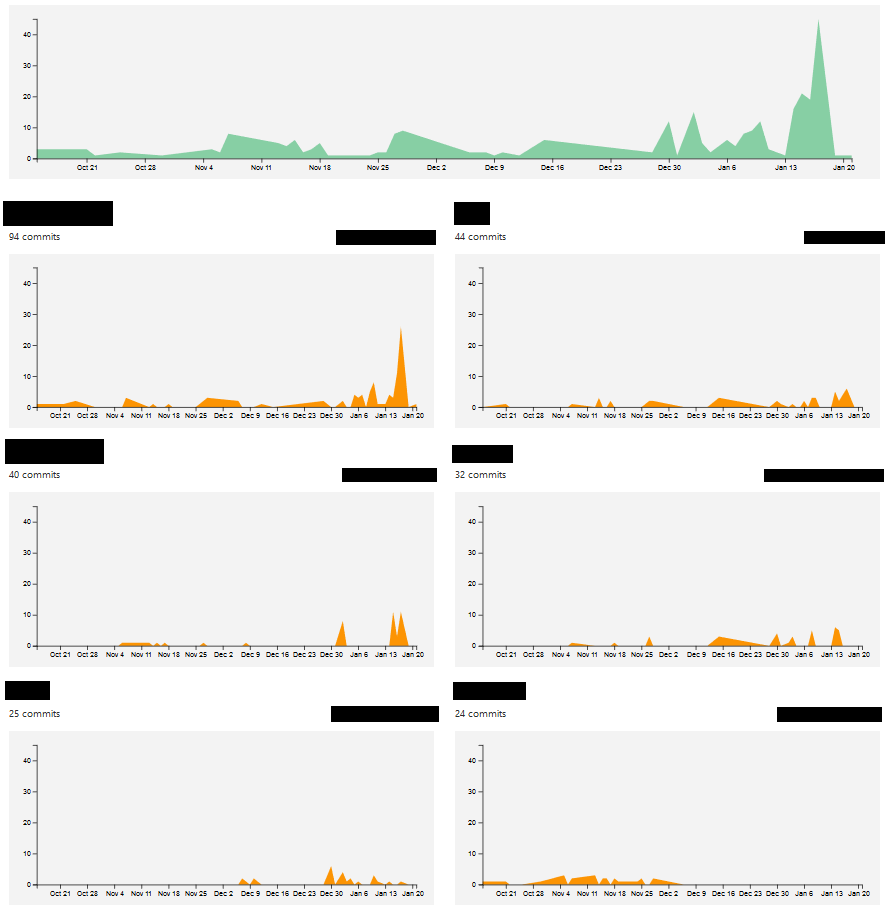
\includegraphics[scale=0.4]{slike/aktivnost.PNG} %veličina slike u odnosu na originalnu datoteku i pozicija slike
	\centering
	\caption{Primjer slike s potpisom}
	\label{fig:promjene}
\end{figure}

\begin{figure}[H]
	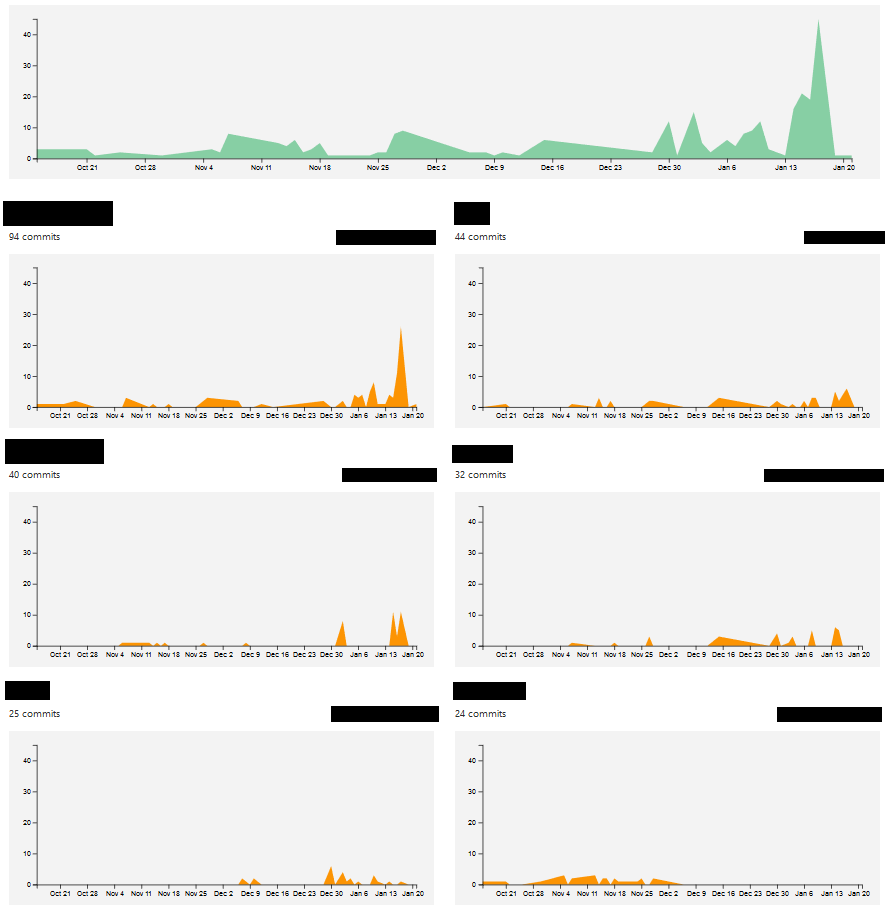
\includegraphics[width=\textwidth]{slike/aktivnost.PNG} %veličina u odnosu na širinu linije
	\caption{Primjer slike s potpisom 2}
	\label{fig:promjene2} %label mora biti drugaciji za svaku sliku
\end{figure}

Referenciranje slike \ref{fig:promjene2} u tekstu.

\eject


	\chapter{Specifikacija programske potpore}

\section{Funkcionalni zahtjevi}

\noindent \textbf{Dionici:}

\begin{packed_enum}

\item Studenti
\item Profesori
\item Asistenti
\item Sveučilište u Zagrebu
\item Razvojni tim

\end{packed_enum}

\noindent \textbf{Aktori i njihovi funkcionalni zahtjevi:}

\begin{packed_enum}
\item  \underbar{Anonimni korisnik (inicijator) može:}

    \begin{packed_enum}

    \item prijaviti se u aplikaciju
    \item stvoriti profil
    \item pretraživati članke
        \begin{packed_enum}

        \item po kategorijama
        \item po naslovu

        \end{packed_enum}
    \item vidjeti određeni članak
    \item podijeliti članak na društvenim mrežama
    \item pregledati tuđe profile

    \end{packed_enum}

\item  \underbar{Prijavljeni korisnik (inicijator) može:}

    \begin{packed_enum}

    \item se odjaviti
    \item stvoriti

        \begin{packed_enum}

        \item članak
        \item komentar na članak

        \end{packed_enum}

    \item urediti

        \begin{packed_enum}

        \item svoj članak
        \item svoj komentar na članak
        \item svoj profil

        \end{packed_enum}

    \item obrisati

        \begin{packed_enum}

        \item svoj članak
        \item svoj komentar na članak

        \end{packed_enum}

    \item vidjeti obavijesti
    \item ocijeniti tuđi članak
    \item pregledati svoj profil
    \item obrisati svoj profil
    \item prijaviti članak

    \end{packed_enum}

\item \underbar{Moderator (inicijator) može:}

    \begin{packed_enum}

    \item zatražiti izmjenu članka
    \item zatražiti izmjenu komentara
    \item obrisati tuđi članak
    \item orisati tuđi komentar
    \item slati obavijesti
    \item privremeno/trajno banati korisnika

    \end{packed_enum}

\item \underbar{Administrator (inicijator) može:}

    \begin{packed_enum}

    \item dodati moderatora/administratora
    \item ukloniti moderatora
    \item odstupiti s mjesta administratora

    \end{packed_enum}

\end{packed_enum}

\eject 

\subsection{Obrasci uporabe}

\subsubsection{Opis obrazaca uporabe}

\noindent \underbar{\textbf{UC1 - Prijava u aplikaciju}}
\begin{packed_item}

\item \textbf{Glavni sudionik:} Anonimni korisnik
\item  \textbf{Cilj:} Prijaviti se u aplikaciju
\item  \textbf{Sudionici:} Baza podataka
\item  \textbf{Preduvjet:} Korisnik je registriran
\item  \textbf{Opis osnovnog tijeka:}

\item[] \begin{packed_enum}

    \item Korisnik ulazi u sučelje za prijavu
    \item Korisnik unosi email adresu i šifru
    \item Provjera valjanosti podataka
    \item Korisnik ulazi u aplikaciju kao prijavljeni korisnik

\end{packed_enum}

\item  \textbf{Opis mogućih odstupanja:}

\item[] \begin{packed_item}

    \item[3.a] Unesena je neispravna email adresa ili šifra

    \item[] \begin{packed_enum}

        \item Sustav obavještava korisnika o neispravnosti unesenih podataka, i predlaže korisniku promjenu unesenih podataka

    \end{packed_enum}

\end{packed_item}

\end{packed_item}

\noindent \underbar{\textbf{UC2 - Stvaranje računa}}
\begin{packed_item}

\item \textbf{Glavni sudionik:} Anonimni korisnik
\item  \textbf{Cilj:} Stvoriti račun
\item  \textbf{Sudionici:} Baza podataka
\item  \textbf{Preduvjet:} -
\item  \textbf{Opis osnovnog tijeka:}

\item[] \begin{packed_enum}

    \item Korisnik ulazi u sučelje za stvaranje računa
    \item Korisnik unosi ime, email adresu i šifru
    \item Provjera valjanosti podataka
    \item Sustav dojavljuje korisniku kako je registracija uspješna

\end{packed_enum}

\item  \textbf{Opis mogućih odstupanja:}

\item[] \begin{packed_item}

    \item[3.a] Račun s već navedenom email adresom već postoji

    \item[] \begin{packed_enum}

        \item Sustav predlaže korisniku promjenu unesene email adrese ili prijavu u postojeći profil pod navedenom adresom

    \end{packed_enum}

\item[3.b] Šifra je preslaba

\item[] \begin{packed_enum}

    \item Sustav predlaže korisniku promjenu unesene šifre

\end{packed_enum}

    \item[3.c] Drugi unos šifre se ne podudara s prvim

    \item[] \begin{packed_enum}

        \item Sustav obavještava korisnika da se šifre razlikuju

    \end{packed_enum}

\end{packed_item}

\end{packed_item}

\noindent \underbar{\textbf{UC3 - Pretraga članaka po kategorijama}}
\begin{packed_item}

\item \textbf{Glavni sudionik:} Anonimni/prijavljeni korisnik
\item  \textbf{Cilj:} Pretražiti članke po kategorijama
\item  \textbf{Sudionici:} Baza podataka
\item  \textbf{Preduvjet:} -
\item  \textbf{Opis osnovnog tijeka:}

\item[] \begin{packed_enum}

    \item Korisnik bira kategorije za pretragu
    \item Baza podataka dohvaća članke sa zadanim kategorijama
    \item Korisniku se prikazuju dohvaćeni članci

\end{packed_enum}

\item  \textbf{Opis mogućih odstupanja:}

\item[] \begin{packed_item}

    \item[2.a] U bazi podataka ne postoji članak sa navedenim kategorijama

    \item[] \begin{packed_enum}

        \item Sustav obavještava korisnika da nije dohvaćen niti jedan članak, te da proba suziti izbor kategorija

    \end{packed_enum}

\end{packed_item}

\end{packed_item}

\noindent \underbar{\textbf{UC4 - Pretraga članaka po naslovu}}
\begin{packed_item}

\item \textbf{Glavni sudionik:} Anonimni/prijavljeni korisnik
\item  \textbf{Cilj:} Pretražiti članke po naslovu
\item  \textbf{Sudionici:} Baza podataka
\item  \textbf{Preduvjet:} -
\item  \textbf{Opis osnovnog tijeka:}

\item[] \begin{packed_enum}

    \item Korisnik unosi tekst za pretragu
    \item Baza podataka dohvaća članke koji sadrže zadani tekst u naslovu
    \item Korisniku se prikazuju dohvaćeni članci

\end{packed_enum}

\item  \textbf{Opis mogućih odstupanja:}

\item[] \begin{packed_item}

    \item[2.a] U bazi podataka ne postoji članak sa danim tekstom u naslovu

    \item[] \begin{packed_enum}

        \item Sustav obavještava korisnika da nije dohvaćen niti jedan članak, te da proba promijeniti tekst za pretragu

    \end{packed_enum}

\end{packed_item}

\end{packed_item}

\noindent \underbar{\textbf{UC5 - Pregledavanje članka}}
\begin{packed_item}

\item \textbf{Glavni sudionik:} Anonimni/prijavljeni korisnik
\item  \textbf{Cilj:} Pregledati određeni članak
\item  \textbf{Sudionici:} Baza podataka
\item  \textbf{Preduvjet:} -
\item  \textbf{Opis osnovnog tijeka:}

\item[] \begin{packed_enum}

    \item Dohvaćanje članka sa baze podataka
    \item Prikaz članka na sučelju

\end{packed_enum}

\end{packed_item}

\noindent \underbar{\textbf{UC6 - Dijeljenje članaka}}
\begin{packed_item}

\item \textbf{Glavni sudionik:} Anonimni/prijavljeni korisnik
\item  \textbf{Cilj:} Podijeliti članak na društvenim mrežama
\item  \textbf{Sudionici:} -
\item  \textbf{Preduvjet:} -
\item  \textbf{Opis osnovnog tijeka:}

\item[] \begin{packed_enum}

    \item Korisnik bira opciju za dijeljenje članka
    \item Korisniku se prikazuje izbornik za društvene mreže
    \item Preusmjeravanje na izabranu društvenu mrežu ili kopiranje adrese u korisnikov međuspremnik

\end{packed_enum}

\item  \textbf{Opis mogućih odstupanja:}

\end{packed_item}

\noindent \underbar{\textbf{UC7 - Pregled profila}}
\begin{packed_item}

\item \textbf{Glavni sudionik:} Anonimni/prijavljeni korisnik
\item  \textbf{Cilj:} Pregledati tuđi profil
\item  \textbf{Sudionici:} Baza podataka
\item  \textbf{Preduvjet:} -
\item  \textbf{Opis osnovnog tijeka:}

\item[] \begin{packed_enum}

    \item Korisnik ulazi na stranicu profila
    \item Baza podataka dohvaća javne podatake profila
    \item Korisniku se prikazuju dohvaćeni podaci profila

\end{packed_enum}

\item  \textbf{Opis mogućih odstupanja:}

\item[] \begin{packed_item}

    \item[2.a] Profil ne postoji, ili je izbrisan

    \item[] \begin{packed_enum}

        \item Korisnik se preusmjerava na matičnu stranicu, sa dojavom da profil ne postoji

    \end{packed_enum}

\end{packed_item}

\end{packed_item}

\noindent \underbar{\textbf{UC8 - Odjava sa aplikacije}}
\begin{packed_item}

\item \textbf{Glavni sudionik:} Prijavljeni korisnik
\item  \textbf{Cilj:} Odjaviti se sa aplikacije
\item  \textbf{Sudionici:} Baza podataka
\item  \textbf{Preduvjet:} Korisnik je prijavljen
\item  \textbf{Opis osnovnog tijeka:}

\item[] \begin{packed_enum}

    \item Korisnik bira opciju za odjavu iz aplikacije
    \item Baza podataka briše zapis o prijavi
    \item Korisnik se preusmjerava na stranicu za anonimnog korisnika

\end{packed_enum}

\end{packed_item}

\noindent \underbar{\textbf{UC9 - Stvaranje članaka}}
\begin{packed_item}

\item \textbf{Glavni sudionik:} Prijavljeni korisnik
\item  \textbf{Cilj:} Stvoriti novi članak
\item  \textbf{Sudionici:} Baza podataka
\item  \textbf{Preduvjet:} Korisnik je prijavljen, korisnik nema ograničen pristup
\item  \textbf{Opis osnovnog tijeka:}

\item[] \begin{packed_enum}

    \item Korisnik otvara sučelje za pisanje članka
    \item Korisnik upisuje tekst članka
    \item Korisnik objavljuje članak
    \item Baza podataka sprema članak
    \item Sustav dojavljuje korisniku da je članak objavljen

\end{packed_enum}

\item  \textbf{Opis mogućih odstupanja:}

\item[] \begin{packed_item}

    \item[3.a] Uneseni tekst je prazan

    \item[] \begin{packed_enum}

        \item Sustav dojavljuje korisniku da tekst ne smije biti prazan

    \end{packed_enum}

\end{packed_item}

\end{packed_item}

\noindent \underbar{\textbf{UC10 - Uređivanje članaka}}
\begin{packed_item}

\item \textbf{Glavni sudionik:} Prijavljeni korisnik
\item  \textbf{Cilj:} Urediti vlastiti članak
\item  \textbf{Sudionici:} Baza podataka
\item  \textbf{Preduvjet:} Korisnik je prijavljen, članak pripada korisniku
\item  \textbf{Opis osnovnog tijeka:}

\item[] \begin{packed_enum}

    \item Korisnik bira opciju za uređivanje članka
    \item Otvara se sučelje za pisanje članka
    \item Korisnik unosi promjene u članak
    \item Korisnik objavljuje članak
    \item Baza podataka sprema promjene članka
    \item Sustav dojavljuje korisniku da je članak uređen

\end{packed_enum}

\item  \textbf{Opis mogućih odstupanja:}

\item[] \begin{packed_item}

    \item[3.a] Članak je prazan/nepromijenjen

    \item[] \begin{packed_enum}

        \item Sustav dojavljuje korisniku da tekst ne smije biti prazan/nepromijenjen

    \end{packed_enum}

\end{packed_item}

\end{packed_item}

\noindent \underbar{\textbf{UC11 - Brisanje vlastitog članka}}
\begin{packed_item}

\item \textbf{Glavni sudionik:} Prijavljeni korisnik
\item  \textbf{Cilj:} Obrisati vlastiti članak
\item  \textbf{Sudionici:} Baza podataka
\item  \textbf{Preduvjet:} Korisnik je prijavljen, članak pripada korisniku
\item  \textbf{Opis osnovnog tijeka:}

\item[] \begin{packed_enum}

    \item Korisnik bira opciju za brisanje članka
    \item Otvara se sučelje za potvrdu brisanja članka
    \item Korisnik potvrđuje brisanje članka
    \item Baza podataka briše članak

\end{packed_enum}

\item  \textbf{Opis mogućih odstupanja:}

\item[] \begin{packed_item}

    \item[3.a] Korisnik nije potvrdio brisanje članka
    \item[] \begin{packed_enum}

        \item Članak se ne briše

    \end{packed_enum}

\end{packed_item}
\end{packed_item}

\noindent \underbar{\textbf{UC12 - Pregled obavijesti}}
\begin{packed_item}

\item \textbf{Glavni sudionik:} Prijavljeni korisnik
\item  \textbf{Cilj:} Pregledati obavijesti
\item  \textbf{Sudionici:} Baza podataka
\item  \textbf{Preduvjet:} Korisnik je prijavljen
\item  \textbf{Opis osnovnog tijeka:}

\item[] \begin{packed_enum}

    \item Korisnik otvara sučelje za prikaz obavijesti
    \item Baza podataka dohvaća obavijesti

\end{packed_enum}

\item  \textbf{Opis mogućih odstupanja:}

\item[] \begin{packed_item}

    \item[2.a] Nema zapisa o obavijestima za korisnika
    \item[] \begin{packed_enum}

        \item Sustav dojavljuje korisniku da nema obavijesti

    \end{packed_enum}

\end{packed_item}
\end{packed_item}

\noindent \underbar{\textbf{UC13 - Ocjenjivanje članaka}}
\begin{packed_item}

\item \textbf{Glavni sudionik:} Prijavljeni korisnik
\item  \textbf{Cilj:} Ocijeniti tuđi članak
\item  \textbf{Sudionici:} Baza podataka
\item  \textbf{Preduvjet:} Korisnik je prijavljen
\item  \textbf{Opis osnovnog tijeka:}

\item[] \begin{packed_enum}

    \item Korisnik ocjenjuje članak jednom od predodređenih ocjena
    \item Baza podataka sprema zapis o ocjeni od korisnika na članak
    \item Sučelje osvježava prikaz o ocjenama članka

\end{packed_enum}

\item  \textbf{Opis mogućih odstupanja:}

\item[] \begin{packed_item}

    \item[2.a] Korisnik je već ostavio ocjenu na članak
    \item[] \begin{packed_enum}

        \item Baza podataka unosi promjene na već postojeći zapis

    \end{packed_enum}

    \item[2.b] Korisnik pokušava ostaviti ocjenu na vlastiti članak
    \item[] \begin{packed_enum}

        \item Sustav dojavljuje korisniku da ne može ocijeniti vlastiti članak

    \end{packed_enum}

\end{packed_item}
\end{packed_item}

\noindent \underbar{\textbf{UC14 - Komentiranje članaka}}
\begin{packed_item}

\item \textbf{Glavni sudionik:} Prijavljeni korisnik
\item  \textbf{Cilj:} Komentirati članak
\item  \textbf{Sudionici:} Baza podataka
\item  \textbf{Preduvjet:} Korisnik je prijavljen, korisnik nema ograničen pristup
\item  \textbf{Opis osnovnog tijeka:}

\item[] \begin{packed_enum}

    \item Korisnik otvara sučelje za pisanje komentara
    \item Korisnik upisuje komentar
    \item Korisnik objavljuje komentar

\end{packed_enum}

\item  \textbf{Opis mogućih odstupanja:}

\item[] \begin{packed_item}

    \item[3.a] Komentar je prazan
    \item[] \begin{packed_enum}

        \item Sustav dojavljuje korisniku da komentar ne smije biti prazan

    \end{packed_enum}

\end{packed_item}

\end{packed_item}

\noindent \underbar{\textbf{UC15 - Brisanje vlastitih komentara}}
\begin{packed_item}

\item \textbf{Glavni sudionik:} Prijavljeni korisnik
\item  \textbf{Cilj:} Obrisati vlastiti komentar na članak
\item  \textbf{Sudionici:} Baza podataka
\item  \textbf{Preduvjet:} Korisnik je prijavljen, komentar pripada korisniku
\item  \textbf{Opis osnovnog tijeka:}

\item[] \begin{packed_enum}

    \item Korisnik bira opciju za brisanje komentara
    \item Otvara se sučelje za potvrdu brisanja komentara
    \item Korisnik potvrđuje brisanje komentara
    \item Baza podataka briše komentar

\end{packed_enum}

\item  \textbf{Opis mogućih odstupanja:}

\item[] \begin{packed_item}

    \item[3.a] Korisnik nije potvrdio brisanje komentara
    \item[] \begin{packed_enum}

        \item Komentar se ne briše

    \end{packed_enum}

\end{packed_item}
\end{packed_item}

\noindent \underbar{\textbf{UC16 - Pregled vlastitog profila}}
\begin{packed_item}

\item \textbf{Glavni sudionik:} Prijavljeni korisnik
\item  \textbf{Cilj:} Pregledati vlastiti profil
\item  \textbf{Sudionici:} Baza podataka
\item  \textbf{Preduvjet:} Korisnik je prijavljen
\item  \textbf{Opis osnovnog tijeka:}

\item[] \begin{packed_enum}

    \item Korisnik bira opciju za pregled profila
    \item Baza podataka dohvaća podatke profila korisnika
    \item Korisniku se prikazuju dohvaćeni podatci

\end{packed_enum}

\end{packed_item}

\noindent \underbar{\textbf{UC17 - Uređivanje profila}}
\begin{packed_item}

\item \textbf{Glavni sudionik:} Prijavljeni korisnik
\item  \textbf{Cilj:} Urediti vlastiti profil
\item  \textbf{Sudionici:} Baza podataka
\item  \textbf{Preduvjet:} Korisnik je prijavljen
\item  \textbf{Opis osnovnog tijeka:}

\item[] \begin{packed_enum}

    \item Korisnik bira opciju za uređivanje profila
    \item Baza podataka dohvaća trenutne podatke profila korisnika
    \item Korisniku se dohvaćeni podatci prikazuju
    \item Korisnik uređuje podatke
    \item Korisnik sprema promjene profila
    \item Baza podataka sprema promjene profila

\end{packed_enum}

\item  \textbf{Opis mogućih odstupanja:}

\item[] \begin{packed_item}

    \item[6.a] Neki od podataka nisu valjani
    \item[] \begin{packed_enum}

        \item Sustav korisniku dojavljuje da profil nije spremljen, te koji su podatci nevaljani

    \end{packed_enum}

\end{packed_item}
\end{packed_item}

\noindent \underbar{\textbf{UC18 - Brisanje profila}}
\begin{packed_item}

\item \textbf{Glavni sudionik:} Prijavljeni korisnik
\item  \textbf{Cilj:} Izbrisati vlastiti profil
\item  \textbf{Sudionici:} Baza podataka
\item  \textbf{Preduvjet:} Korisnik je prijavljen
\item  \textbf{Opis osnovnog tijeka:}

\item[] \begin{packed_enum}

    \item Korisnik bira opciju za brisanje profila
    \item Otvara se sučelje za potvrdu brisanja profila
    \item Korisnik potvrđuje brisanje profila
    \item Baza podataka briše zapis o korisničkom profilu

\end{packed_enum}

\item  \textbf{Opis mogućih odstupanja:}

\item[] \begin{packed_item}

    \item[3.a] Korisnik nije potvrdio brisanje profila
    \item[] \begin{packed_enum}

        \item Profil se ne briše

    \end{packed_enum}

\end{packed_item}
\end{packed_item}

\noindent \underbar{\textbf{UC19 - Prijavljivanje članaka}}
\begin{packed_item}

\item \textbf{Glavni sudionik:} Prijavljeni korisnik
\item  \textbf{Cilj:} Prijaviti neprimjeren članak
\item  \textbf{Sudionici:} Baza podataka
\item  \textbf{Preduvjet:} Korisnik je prijavljen
\item  \textbf{Opis osnovnog tijeka:}

\item[] \begin{packed_enum}

    \item Korisnik bira opciju za prijavljivanje članka
    \item Korisniku se prikazuje sučelje za opis neprimjerenog sadržaja
    \item Korisnik unosi podatke
    \item Korisnik prijavljuje članak
    \item Baza podataka sprema prijavu članka

\end{packed_enum}

\item  \textbf{Opis mogućih odstupanja:}

\item[] \begin{packed_item}

    \item[5.a] Podatci su neispravni ili nedostaju
    \item[] \begin{packed_enum}

        \item Sustav dojavljuje korisniku da su podatci neispravni ili nedostaju

    \end{packed_enum}

\end{packed_item}
\end{packed_item}

\noindent \underbar{\textbf{UC20 - Pregledavanje komentara}}
\begin{packed_item}

\item \textbf{Glavni sudionik:} Anonimni/prijavljeni korisnik
\item  \textbf{Cilj:} Pregledati komentare na nečiji članak
\item  \textbf{Sudionici:} Baza podataka
\item  \textbf{Preduvjet:} -
\item  \textbf{Opis osnovnog tijeka:}

\item[] \begin{packed_enum}

    \item Korisnik bira opciju za prikaz komentara na članku
    \item Baza podataka dohvaća komentare na članak
    \item Korisniku se prikazuju dohvaćeni komentari

\end{packed_enum}

\item  \textbf{Opis mogućih odstupanja:}

\item[] \begin{packed_item}

    \item[2.a] Na članku nema komentara
    \item[] \begin{packed_enum}

        \item Sustav dojavljuje korisniku da objava nema komentara

    \end{packed_enum}

\end{packed_item}
\end{packed_item}

\noindent \underbar{\textbf{UC21 - Prijavljivanje komentara}}
\begin{packed_item}

\item \textbf{Glavni sudionik:} Prijavljeni korisnik
\item  \textbf{Cilj:} Prijaviti neprimjeren komentar
\item  \textbf{Sudionici:} Baza podataka
\item  \textbf{Preduvjet:} Korisnik je prijavljen
\item  \textbf{Opis osnovnog tijeka:}

\item[] \begin{packed_enum}

    \item Korisnik bira opciju za prijavljivanje komentara
    \item Korisniku se prikazuje sučelje za opis neprimjerenog sadržaja
    \item Korisnik unosi podatke
    \item Korisnik prijavljuje komentar
    \item Baza podataka sprema prijavu komentara

\end{packed_enum}

\item  \textbf{Opis mogućih odstupanja:}

\item[] \begin{packed_item}

    \item[5.a] Podatci su neispravni ili nedostaju
    \item[] \begin{packed_enum}

        \item Sustav dojavljuje korisniku da su podatci neispravni ili nedostaju

    \end{packed_enum}

\end{packed_item}
\end{packed_item}

\noindent \underbar{\textbf{UC22 - Izmjena nečijeg članka}}
\begin{packed_item}

\item \textbf{Glavni sudionik:} Moderator
\item  \textbf{Cilj:} Predložiti drugom korisniku izmjenu članka
\item  \textbf{Sudionici:} Baza podataka, prijavljeni korisnik
\item  \textbf{Preduvjet:} -
\item  \textbf{Opis osnovnog tijeka:}

\item[] \begin{packed_enum}

    \item Moderator bira opciju za izmjenu nečijeg članka
    \item Moderator unosi poruku korisniku i/ili predloženu izmjenu
    \item Moderator šalje obavijest korisniku
    \item Baza podataka stvara zapis obavijesti s porukom za korisnika

\end{packed_enum}

\end{packed_item}

\noindent \underbar{\textbf{UC23 - Izmjena nečijeg komentara}}
\begin{packed_item}

\item \textbf{Glavni sudionik:} Moderator
\item  \textbf{Cilj:} Predložiti drugom korisniku izmjenu komentara
\item  \textbf{Sudionici:} Baza podataka, prijavljeni korisnik
\item  \textbf{Preduvjet:} -
\item  \textbf{Opis osnovnog tijeka:}

\item[] \begin{packed_enum}

    \item Moderator bira opciju za izmjenu nečijeg komentara
    \item Moderator unosi poruku korisniku i/ili predloženu komentara
    \item Moderator šalje obavijest korisniku
    \item Baza podataka stvara zapis obavijesti s porukom za korisnika

\end{packed_enum}

\end{packed_item}

\noindent \underbar{\textbf{UC24 - Brisanje članka}}
\begin{packed_item}

\item \textbf{Glavni sudionik:} Moderator
\item  \textbf{Cilj:} Obrisati članak nekog korisnika
\item  \textbf{Sudionici:} Baza podataka, prijavljeni korisnik
\item  \textbf{Preduvjet:} -
\item  \textbf{Opis osnovnog tijeka:}

\item[] \begin{packed_enum}

    \item Moderator bira opciju za brisanje članka
    \item Moderatoru se prikazuje sučelje za brisanje članka
    \item Moderator unosi dodatne informacije u vezi brisanja članka
    \item Moderator potvrđuje brisanje članka
    \item Baza podataka briše zapis članka i stvara zapis obavijesti o brisanju članka za korisnika

\end{packed_enum}

\item  \textbf{Opis mogućih odstupanja:}

\item[] \begin{packed_item}

    \item[4.a] Moderator nije potvrdio brisanje članka
    \item[] \begin{packed_enum}

        \item Članak se ne briše

    \end{packed_enum}

\end{packed_item}
\end{packed_item}

\noindent \underbar{\textbf{UC25 - Brisanje komentara}}
\begin{packed_item}

\item \textbf{Glavni sudionik:} Moderator
\item  \textbf{Cilj:} Obrisati komentar nekog korisnika
\item  \textbf{Sudionici:} Baza podataka, prijavljeni korisnik
\item  \textbf{Preduvjet:} -
\item  \textbf{Opis osnovnog tijeka:}

\item[] \begin{packed_enum}

    \item Moderator bira opciju za brisanje komentara
    \item Moderatoru se prikazuje sučelje za brisanje komentara
    \item Moderator unosi dodatne informacije u vezi brisanja komentara
    \item Moderator potvrđuje brisanje komentara
    \item Baza podataka briše zapis članka i stvara zapis obavijesti o brisanju komentara za korisnika

\end{packed_enum}

\item  \textbf{Opis mogućih odstupanja:}

\item[] \begin{packed_item}

    \item[4.a] Moderator nije potvrdio brisanje komentara
    \item[] \begin{packed_enum}

        \item Komentar se ne briše

    \end{packed_enum}

\end{packed_item}
\end{packed_item}

\noindent \underbar{\textbf{UC26 - Slanje obavijesti}}
\begin{packed_item}

\item \textbf{Glavni sudionik:} Moderator
\item  \textbf{Cilj:} Poslati obavijest jednom ili više korisnika
\item  \textbf{Sudionici:} Baza podataka, prijavljeni korisnik
\item  \textbf{Preduvjet:} -
\item  \textbf{Opis osnovnog tijeka:}

\item[] \begin{packed_enum}

    \item Moderator bira opciju za slanje obavijesti
    \item Moderatoru se prikazuje sučelje za slanje obavijesti
    \item Moderator unosi grupu korisnika kojoj šalje obavijesti i sadržaj obavijesti
    \item Moderator šalje obavijest korisnicima
    \item U bazi podataka se stvara zapis o obavijesti za sve navedene korisnike

\end{packed_enum}

\item  \textbf{Opis mogućih odstupanja:}

\item[] \begin{packed_item}

    \item[5.a] Jedno od unesenih polja je prazno
    \item[] \begin{packed_enum}

        \item Sustav dojavljuje moderatoru da treba ispuniti prazno polje

    \end{packed_enum}

\end{packed_item}
\end{packed_item}

\noindent \underbar{\textbf{UC27 - Bananje korisnika}}
\begin{packed_item}

\item \textbf{Glavni sudionik:} Moderator
\item  \textbf{Cilj:} Zabraniti pristup korisniku na neke funkcionalnosti aplikacije
\item  \textbf{Sudionici:} Baza podataka, korisnik
\item  \textbf{Preduvjet:} Korisnik nije prethodno dobio ograničenje pristupa
\item  \textbf{Opis osnovnog tijeka:}

\item[] \begin{packed_enum}

    \item Moderator bira opciju za bananje korisnika
    \item Moderatoru se prikazuje sučelje za bananje korisnika
    \item Moderator unosi dodatne informacije o banu
    \item Moderator potvrđuje bananje korisnika
    \item Baza podataka sprema zapis o banu korisnika i obavijesti za korisnika o banu

\end{packed_enum}

\item  \textbf{Opis mogućih odstupanja:}

\item[] \begin{packed_item}

    \item[4.a] Moderator nije potvrdio bananje korisnika
    \item[] \begin{packed_enum}

        \item Korisnik se ne bana

    \end{packed_enum}

\end{packed_item}
\end{packed_item}

\noindent \underbar{\textbf{UC28 - Dodavanje privilegiranog korisnika}}
\begin{packed_item}

\item \textbf{Glavni sudionik:} Administrator
\item  \textbf{Cilj:} Dodati korisnika na mjesto moderatora ili administratora
\item  \textbf{Sudionici:} Baza podataka, prijavljeni korisnik ili moderator
\item  \textbf{Preduvjet:} Korisnik nije prethodno bio privilegiran
\item  \textbf{Opis osnovnog tijeka:}

\item[] \begin{packed_enum}

    \item Administrator bira opciju za promociju korisnika ili moderatora
    \item Administratoru se prikazuje sučelje za promociju korisnika ili moderatora
    \item Administrator bira želi li korisnika promovirati na moderatora i administratora
    \item Administrator potvrđuje promociju
    \item Baza podataka sprema novu poziciju korisnika i zapis o obavijesti o promociji korisnika

\end{packed_enum}

\item  \textbf{Opis mogućih odstupanja:}

\item[] \begin{packed_item}

    \item[4.a] Administrator nije potvrdio promociju korisnika
    \item[] \begin{packed_enum}

        \item Korisniku ostaju iste ovlasti koje je imao

    \end{packed_enum}

\end{packed_item}
\end{packed_item}

\noindent \underbar{\textbf{UC29 - Uklanjanje moderatora}}
\begin{packed_item}

\item \textbf{Glavni sudionik:} Administrator
\item  \textbf{Cilj:} Ukloniti korisniku moderatorske ovlasti
\item  \textbf{Sudionici:} Baza podataka, moderator
\item  \textbf{Preduvjet:} -
\item  \textbf{Opis osnovnog tijeka:}

\item[] \begin{packed_enum}

    \item Administrator bira opciju za uklanjanje moderatora
    \item Administratoru se prikazuje sučelje za potvrdu uklanjanja moderatora
    \item Administrator potvrđuje uklanjanje moderatora
    \item Baza podataka sprema novu poziciju moderatora kao korisnika i zapis o obavijesti gubitka moderatorskih ovlasti

\end{packed_enum}

\item  \textbf{Opis mogućih odstupanja:}

\item[] \begin{packed_item}

    \item[3.a] Administrator nije potvrdio uklanjanje moderatora
    \item[] \begin{packed_enum}

        \item Moderatoru ostaju iste ovlasti koje je imao

    \end{packed_enum}

\end{packed_item}
\end{packed_item}

\noindent \underbar{\textbf{UC30 - Odstupanje s mjesta administratora}}
\begin{packed_item}

\item \textbf{Glavni sudionik:} Administrator
\item  \textbf{Cilj:} Ukloniti sebi administratorske ovlasti
\item  \textbf{Sudionici:} Baza podataka
\item  \textbf{Preduvjet:} -
\item  \textbf{Opis osnovnog tijeka:}

\item[] \begin{packed_enum}

    \item Administrator bira opciju za odstupanje s mjesta administratora
    \item Administratoru se prikazuje sučelje za potvrdu za odstupanje
    \item Administrator potvrđuje odstupanje
    \item Baza podataka sprema novu poziciju administratora

\end{packed_enum}

\item  \textbf{Opis mogućih odstupanja:}

\item[] \begin{packed_item}

    \item[3.a] Administrator nije potvrdio odstupanje
    \item[] \begin{packed_enum}

        \item Administratoru ostaju iste ovlasti koje je imao

    \end{packed_enum}

\end{packed_item}
\end{packed_item}

\subsubsection{Dijagrami obrazaca uporabe}

\begin{figure}[H]
	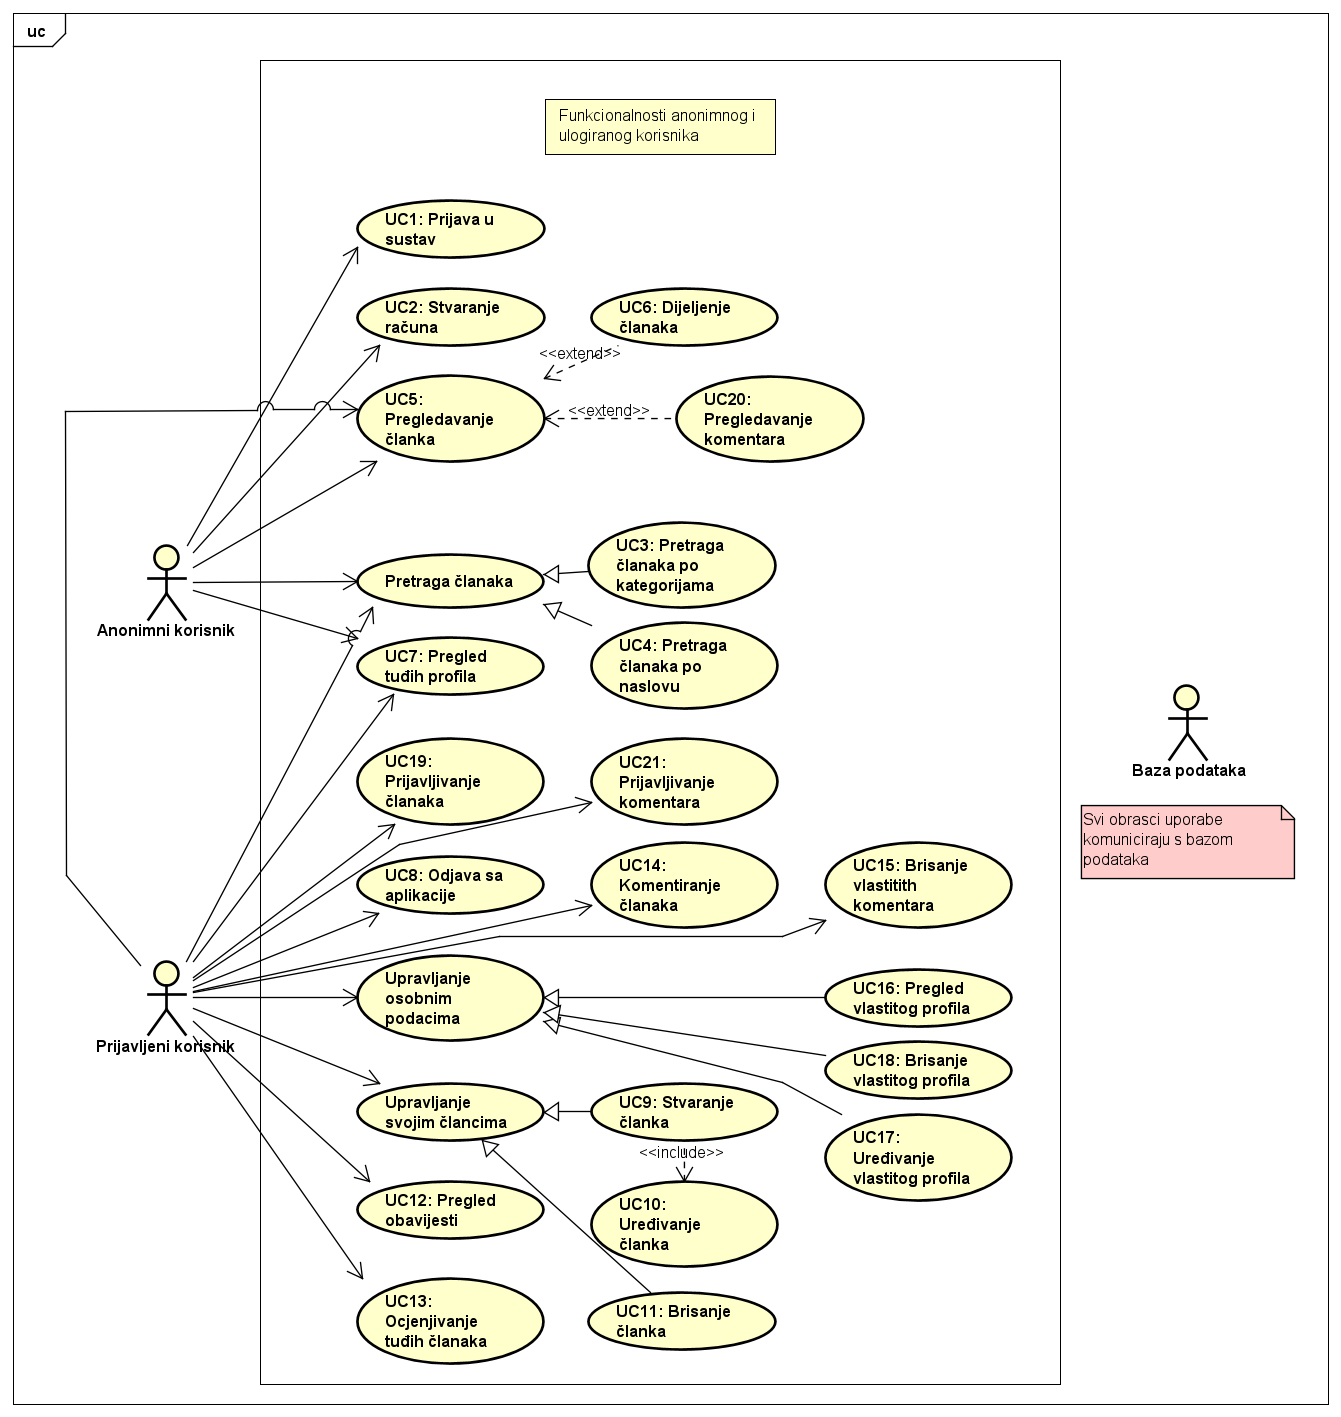
\includegraphics[scale=0.4]{slike/DijagramObrazacaUporabe1.PNG}
	\centering
	\caption{Dijagram obrasca uporabe, funkcionalnost anonimnog i prijavljenog korisnika}
	\label{fig:obrazac_uporabe1}
\end{figure}

\eject		

\begin{figure}[H]
	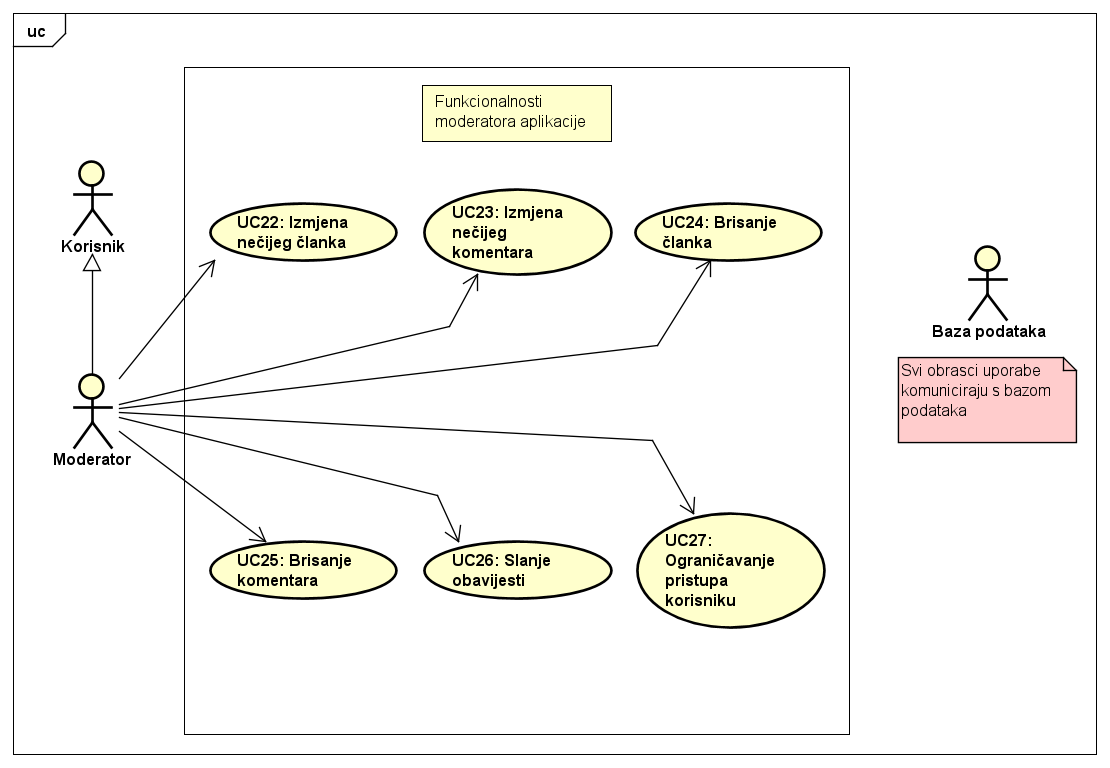
\includegraphics[scale=0.4]{slike/DijagramObrazacaUporabe2.PNG}
	\centering
	\caption{Dijagram obrasca uporabe, funkcionalnost moderatora sustava}
	\label{fig:obrazac_uporabe2}
\end{figure}

\begin{figure}[H]
	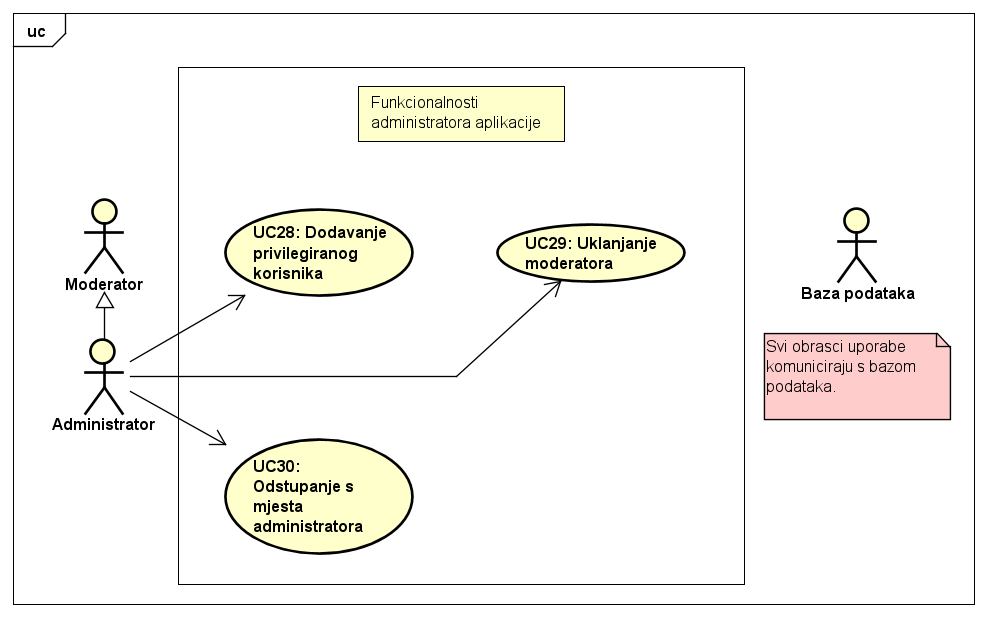
\includegraphics[scale=0.4]{slike/DijagramObrazacaUporabe3.PNG}
	\centering
	\caption{Dijagram obrasca uporabe, funkcionalnost administratora sustava}
	\label{fig:obrazac_uporabe3}
\end{figure}

\eject	

\subsection{Sekvencijski dijagrami}

\textbf{\textit{dio 1. revizije}}\\

\textit{Nacrtati sekvencijske dijagrame koji modeliraju najvažnije dijelove sustava (max. 4 dijagrama). Ukoliko postoji nedoumica oko odabira, razjasniti s asistentom. Uz svaki dijagram napisati detaljni opis dijagrama.}
\eject

\section{Ostali zahtjevi}

\textbf{\textit{dio 1. revizije}}\\

\textit{Nefunkcionalni zahtjevi i zahtjevi domene primjene dopunjuju funkcionalne zahtjeve. Oni opisuju \textbf{kako se sustav treba ponašati} i koja \textbf{ograničenja} treba poštivati (performanse, korisničko iskustvo, pouzdanost, standardi kvalitete, sigurnost...). Primjeri takvih zahtjeva u Vašem projektu mogu biti: podržani jezici korisničkog sučelja, vrijeme odziva, najveći mogući podržani broj korisnika, podržane web/mobilne platforme, razina zaštite (protokoli komunikacije, kriptiranje...)... Svaki takav zahtjev potrebno je navesti u jednoj ili dvije rečenice.}

	\chapter{Arhitektura i dizajn sustava}
		
		\textbf{\textit{dio 1. revizije}}\\

		\textit{ Potrebno je opisati stil arhitekture te identificirati: podsustave, preslikavanje na radnu platformu, spremišta podataka, mrežne protokole, globalni upravljački tok i sklopovsko-programske zahtjeve. Po točkama razraditi i popratiti odgovarajućim skicama:}
	\begin{itemize}
		\item 	\textit{izbor arhitekture temeljem principa oblikovanja pokazanih na predavanjima (objasniti zašto ste baš odabrali takvu arhitekturu)}
		\item 	\textit{organizaciju sustava s najviše razine apstrakcije (npr. klijent-poslužitelj, baza podataka, datotečni sustav, grafičko sučelje)}
		\item 	\textit{organizaciju aplikacije (npr. slojevi frontend i backend, MVC arhitektura) }		
	\end{itemize}

	
		

		

				
		\section{Baza podataka}
			
			\textbf{\textit{dio 1. revizije}}\\
			
		\textit{Potrebno je opisati koju vrstu i implementaciju baze podataka ste odabrali, glavne komponente od kojih se sastoji i slično.}
		
			\subsection{Opis tablica}
			

				\textit{Svaku tablicu je potrebno opisati po zadanom predlošku. Lijevo se nalazi točno ime varijable u bazi podataka, u sredini se nalazi tip podataka, a desno se nalazi opis varijable. Svjetlozelenom bojom označite primarni ključ. Svjetlo plavom označite strani ključ}
				
				
				\begin{longtblr}[
					label=none,
					entry=none
					]{
						width = \textwidth,
						colspec={|X[6,l]|X[6, l]|X[20, l]|}, 
						rowhead = 1,
					} %definicija širine tablice, širine stupaca, poravnanje i broja redaka naslova tablice
					\hline \SetCell[c=3]{c}{\textbf{korisnik - ime tablice}}	 \\ \hline[3pt]
					\SetCell{LightGreen}IDKorisnik & INT	&  	Lorem ipsum dolor sit amet, consectetur adipiscing elit, sed do eiusmod  	\\ \hline
					korisnickoIme	& VARCHAR &   	\\ \hline 
					email & VARCHAR &   \\ \hline 
					ime & VARCHAR	&  		\\ \hline 
					\SetCell{LightBlue} primjer	& VARCHAR &   	\\ \hline 
				\end{longtblr}
				
				
			
			\subsection{Dijagram baze podataka}
				\textit{ U ovom potpoglavlju potrebno je umetnuti dijagram baze podataka. Primarni i strani ključevi moraju biti označeni, a tablice povezane. Bazu podataka je potrebno normalizirati. Podsjetite se kolegija "Baze podataka".}
			
			\eject
			
			
		\section{Dijagram razreda}
		
			\textit{Potrebno je priložiti dijagram razreda s pripadajućim opisom. Zbog preglednosti je moguće dijagram razlomiti na više njih, ali moraju biti grupirani prema sličnim razinama apstrakcije i srodnim funkcionalnostima.}\\
			
			\textbf{\textit{dio 1. revizije}}\\
			
			\textit{Prilikom prve predaje projekta, potrebno je priložiti potpuno razrađen dijagram razreda vezan uz \textbf{generičku funkcionalnost} sustava. Ostale funkcionalnosti trebaju biti idejno razrađene u dijagramu sa sljedećim komponentama: nazivi razreda, nazivi metoda i vrste pristupa metodama (npr. javni, zaštićeni), nazivi atributa razreda, veze i odnosi između razreda.}\\
			
			\textbf{\textit{dio 2. revizije}}\\			
			
			\textit{Prilikom druge predaje projekta dijagram razreda i opisi moraju odgovarati stvarnom stanju implementacije}
			
			
			
			\eject
		
		\section{Dijagram stanja}
			
			
			\textbf{\textit{dio 2. revizije}}\\
			
			\textit{Potrebno je priložiti dijagram stanja i opisati ga. Dovoljan je jedan dijagram stanja koji prikazuje \textbf{značajan dio funkcionalnosti} sustava. Na primjer, stanja korisničkog sučelja i tijek korištenja neke ključne funkcionalnosti jesu značajan dio sustava, a registracija i prijava nisu. }
			
			
			\eject 
		
		\section{Dijagram aktivnosti}
			
			\textbf{\textit{dio 2. revizije}}\\
			
			 \textit{Potrebno je priložiti dijagram aktivnosti s pripadajućim opisom. Dijagram aktivnosti treba prikazivati značajan dio sustava.}
			
			\eject
		\section{Dijagram komponenti}
		
			\textbf{\textit{dio 2. revizije}}\\
		
			 \textit{Potrebno je priložiti dijagram komponenti s pripadajućim opisom. Dijagram komponenti treba prikazivati strukturu cijele aplikacije.}
	\chapter{Implementacija i korisničko sučelje}
		
		
		\section{Korištene tehnologije i alati}
		
			\textbf{\textit{dio 2. revizije}}
			
			 \textit{Detaljno navesti sve tehnologije i alate koji su primijenjeni pri izradi dokumentacije i aplikacije. Ukratko ih opisati, te navesti njihovo značenje i mjesto primjene. Za svaki navedeni alat i tehnologiju je potrebno \textbf{navesti internet poveznicu} gdje se mogu preuzeti ili više saznati o njima}.
			
			
			\eject 
		
	
		\section{Ispitivanje programskog rješenja}
			
			\textbf{\textit{dio 2. revizije}}\\
			
			 \textit{U ovom poglavlju je potrebno opisati provedbu ispitivanja implementiranih funkcionalnosti na razini komponenti i na razini cijelog sustava s prikazom odabranih ispitnih slučajeva. Studenti trebaju ispitati temeljnu funkcionalnost i rubne uvjete.}
	
			
			\subsection{Ispitivanje komponenti}
			\textit{Potrebno je provesti ispitivanje jedinica (engl. unit testing) nad razredima koji implementiraju temeljne funkcionalnosti. Razraditi \textbf{minimalno 6 ispitnih slučajeva} u kojima će se ispitati redovni slučajevi, rubni uvjeti te izazivanje pogreške (engl. exception throwing). Poželjno je stvoriti i ispitni slučaj koji koristi funkcionalnosti koje nisu implementirane. Potrebno je priložiti izvorni kôd svih ispitnih slučajeva te prikaz rezultata izvođenja ispita u razvojnom okruženju (prolaz/pad ispita). }
			
			
			
			\subsection{Ispitivanje sustava}
			
			 \textit{Potrebno je provesti i opisati ispitivanje sustava koristeći radni okvir Selenium\footnote{\url{https://www.seleniumhq.org/}}. Razraditi \textbf{minimalno 4 ispitna slučaja} u kojima će se ispitati redovni slučajevi, rubni uvjeti te poziv funkcionalnosti koja nije implementirana/izaziva pogrešku kako bi se vidjelo na koji način sustav reagira kada nešto nije u potpunosti ostvareno. Ispitni slučaj se treba sastojati od ulaza (npr. korisničko ime i lozinka), očekivanog izlaza ili rezultata, koraka ispitivanja i dobivenog izlaza ili rezultata.\\ }
			 
			 \textit{Izradu ispitnih slučajeva pomoću radnog okvira Selenium moguće je provesti pomoću jednog od sljedeća dva alata:}
			 \begin{itemize}
			 	\item \textit{dodatak za preglednik \textbf{Selenium IDE} - snimanje korisnikovih akcija radi automatskog ponavljanja ispita	}
			 	\item \textit{\textbf{Selenium WebDriver} - podrška za pisanje ispita u jezicima Java, C\#, PHP koristeći posebno programsko sučelje.}
			 \end{itemize}
		 	\textit{Detalji o korištenju alata Selenium bit će prikazani na posebnom predavanju tijekom semestra.}
			
			\eject 
		
		
		\section{Dijagram razmještaja}
			
			\textbf{\textit{dio 2. revizije}}
			
			 \textit{Potrebno je umetnuti \textbf{specifikacijski} dijagram razmještaja i opisati ga. Moguće je umjesto specifikacijskog dijagrama razmještaja umetnuti dijagram razmještaja instanci, pod uvjetom da taj dijagram bolje opisuje neki važniji dio sustava.}
			
			\eject 
		
		\section{Upute za puštanje u pogon}
		
			\textbf{\textit{dio 2. revizije}}\\
		
			 \textit{U ovom poglavlju potrebno je dati upute za puštanje u pogon (engl. deployment) ostvarene aplikacije. Na primjer, za web aplikacije, opisati postupak kojim se od izvornog kôda dolazi do potpuno postavljene baze podataka i poslužitelja koji odgovara na upite korisnika. Za mobilnu aplikaciju, postupak kojim se aplikacija izgradi, te postavi na neku od trgovina. Za stolnu (engl. desktop) aplikaciju, postupak kojim se aplikacija instalira na računalo. Ukoliko mobilne i stolne aplikacije komuniciraju s poslužiteljem i/ili bazom podataka, opisati i postupak njihovog postavljanja. Pri izradi uputa preporučuje se \textbf{naglasiti korake instalacije uporabom natuknica} te koristiti što je više moguće \textbf{slike ekrana} (engl. screenshots) kako bi upute bile jasne i jednostavne za slijediti.}
			
			
			 \textit{Dovršenu aplikaciju potrebno je pokrenuti na javno dostupnom poslužitelju. Studentima se preporuča korištenje neke od sljedećih besplatnih usluga: \href{https://aws.amazon.com/}{Amazon AWS}, \href{https://azure.microsoft.com/en-us/}{Microsoft Azure} ili \href{https://www.heroku.com/}{Heroku}. Mobilne aplikacije trebaju biti objavljene na F-Droid, Google Play ili Amazon App trgovini.}
			
			
			\eject 
	\chapter{Zaključak i budući rad}
		
		\textbf{\textit{dio 2. revizije}}\\
		
		 \textit{U ovom poglavlju potrebno je napisati osvrt na vrijeme izrade projektnog zadatka, koji su tehnički izazovi prepoznati, jesu li riješeni ili kako bi mogli biti riješeni, koja su znanja stečena pri izradi projekta, koja bi znanja bila posebno potrebna za brže i kvalitetnije ostvarenje projekta i koje bi bile perspektive za nastavak rada u projektnoj grupi.}
		
		 \textit{Potrebno je točno popisati funkcionalnosti koje nisu implementirane u ostvarenoj aplikaciji.}
		
		\eject 
	\chapter*{Popis literature}
		\addcontentsline{toc}{chapter}{Popis literature}
		
		\begin{enumerate}
			
			
			\item  Programsko inženjerstvo, FER ZEMRIS, \url{http://www.fer.hr/predmet/proinz}
			
			\item  I. Sommerville, "Software engineering", 8th ed, Addison Wesley, 2007.
			
			\item  T.C.Lethbridge, R.Langaniere, "Object-Oriented Software Engineering", 2nd ed. McGraw-Hill, 2005.
			
			\item  I. Marsic, Software engineering book``, Department of Electrical and Computer Engineering, Rutgers University, \url{http://www.ece.rutgers.edu/~marsic/books/SE}
			
			\item  The Unified Modeling Language, \url{https://www.uml-diagrams.org/}
			
			\item  Astah Community, \url{http://astah.net/editions/uml-new}
			
			\item React dokumentacija, \url{https://react.dev/learn}
			
			\item Spring Boot dokumentacija, \url{https://docs.spring.io/}
			
			\item Docker dokumentacija, \url{https://docs.docker.com/}
			
			\item MDN web docs, \url{https://developer.mozilla.org/}
		\end{enumerate}
		
		 
	
	
	\begingroup
	\renewcommand*\listfigurename{Indeks slika i dijagrama}
	%\renewcommand*\listtablename{Indeks tablica}
	%\let\clearpage\relax
	\listoffigures
	%\vspace{10mm}
	%\listoftables
	\endgroup
	\addcontentsline{toc}{chapter}{Indeks slika i dijagrama}


	
	\eject 
		
	\chapter*{Dodatak: Prikaz aktivnosti grupe}
		\addcontentsline{toc}{chapter}{Dodatak: Prikaz aktivnosti grupe}
		
		\section*{Dnevnik sastajanja}
		
		\textbf{\textit{Kontinuirano osvježavanje}}\\
		
		 \textit{U ovom dijelu potrebno je redovito osvježavati dnevnik sastajanja prema predlošku.}
		
		\begin{packed_enum}
			\item  sastanak
			
			\item[] \begin{packed_item}
				\item Datum: u ovom formatu: \today
				\item Prisustvovali: I.Prezime, I.Prezime
				\item Teme sastanka:
				\begin{packed_item}
					\item  opis prve teme
					\item  opis druge teme
				\end{packed_item}
			\end{packed_item}
			
			\item  sastanak
			\item[] \begin{packed_item}
				\item Datum: u ovom formatu: \today
				\item Prisustvovali: I.Prezime, I.Prezime
				\item Teme sastanka:
				\begin{packed_item}
					\item  opis prve teme
					\item  opis druge teme
				\end{packed_item}
			\end{packed_item}
			
			%
			
		\end{packed_enum}
		
		\eject
		\section*{Tablica aktivnosti}
		
			\textbf{\textit{Kontinuirano osvježavanje}}\\
			
			 \textit{Napomena: Doprinose u aktivnostima treba navesti u satima po članovima grupe po aktivnosti.}

			\begin{longtblr}[
					label=none,
				]{
					vlines,hlines,
					width = \textwidth,
					colspec={X[7, l]X[1, c]X[1, c]X[1, c]X[1, c]X[1, c]X[1, c]X[1, c]}, 
					vline{1} = {1}{text=\clap{}},
					hline{1} = {1}{text=\clap{}},
					rowhead = 1,
				} 
			
				\SetCell[c=1]{c}{} & \SetCell[c=1]{c}{\rotatebox{90}{\textbf{Ime Prezime voditelja}}} & \SetCell[c=1]{c}{\rotatebox{90}{\textbf{Ime Prezime }}} &	\SetCell[c=1]{c}{\rotatebox{90}{\textbf{Ime Prezime }}} & \SetCell[c=1]{c}{\rotatebox{90}{\textbf{Ime Prezime }}} &	\SetCell[c=1]{c}{\rotatebox{90}{\textbf{Ime Prezime }}} & \SetCell[c=1]{c}{\rotatebox{90}{\textbf{Ime Prezime }}} &	\SetCell[c=1]{c}{\rotatebox{90}{\textbf{Ime Prezime }}} \\  
				Upravljanje projektom 		&  &  &  &  &  &  & \\ 
				Opis projektnog zadatka 	&  &  &  &  &  &  & \\ 
				
				Funkcionalni zahtjevi       &  &  &  &  &  &  &  \\ 
				Opis pojedinih obrazaca 	&  &  &  &  &  &  &  \\ 
				Dijagram obrazaca 			&  &  &  &  &  &  &  \\ 
				Sekvencijski dijagrami 		&  &  &  &  &  &  &  \\ 
				Opis ostalih zahtjeva 		&  &  &  &  &  &  &  \\ 

				Arhitektura i dizajn sustava	 &  &  &  &  &  &  &  \\ 
				Baza podataka				&  &  &  &  &  &  &   \\ 
				Dijagram razreda 			&  &  &  &  &  &  &   \\ 
				Dijagram stanja				&  &  &  &  &  &  &  \\ 
				Dijagram aktivnosti 		&  &  &  &  &  &  &  \\ 
				Dijagram komponenti			&  &  &  &  &  &  &  \\ 
				Korištene tehnologije i alati 		&  &  &  &  &  &  &  \\ 
				Ispitivanje programskog rješenja 	&  &  &  &  &  &  &  \\ 
				Dijagram razmještaja			&  &  &  &  &  &  &  \\ 
				Upute za puštanje u pogon 		&  &  &  &  &  &  &  \\  
				Dnevnik sastajanja 			&  &  &  &  &  &  &  \\ 
				Zaključak i budući rad 		&  &  &  &  &  &  &  \\  
				Popis literature 			&  &  &  &  &  &  &  \\  
				&  &  &  &  &  &  &  \\ \hline 
				\textit{Dodatne stavke kako ste podijelili izradu aplikacije} 			&  &  &  &  &  &  &  \\ 
				\textit{npr. izrada početne stranice} 				&  &  &  &  &  &  &  \\  
				\textit{izrada baze podataka} 		 			&  &  &  &  &  &  & \\  
				\textit{spajanje s bazom podataka} 							&  &  &  &  &  &  &  \\ 
				\textit{back end} 							&  &  &  &  &  &  &  \\  
				 							&  &  &  &  &  &  &\\ 
			\end{longtblr}
					
					
		\eject
		\section*{Dijagrami pregleda promjena}
		
		\textbf{\textit{dio 2. revizije}}\\
		
		\textit{Prenijeti dijagram pregleda promjena nad datotekama projekta. Potrebno je na kraju projekta generirane grafove s gitlaba prenijeti u ovo poglavlje dokumentacije. Dijagrami za vlastiti projekt se mogu preuzeti s gitlab.com stranice, u izborniku Repository, pritiskom na stavku Contributors.}
		
	


\end{document} %naredbe i tekst nakon ove naredbe ne ulaze u izgrađen dokument 


